\textbf{Simulado 2}

\textbf{Questão 1:}

\textbf{Carmen Perez: Fazendas têm diversas estratégias para coibir
incêndios}

A Especialista CNN em agronegócio explicou como os produtores rurais
evitam os danos causados por incêndios durante a época de seca.

No período entre julho e setembro, a ocorrência de queimadas se torna
mais frequente, por conta da estiagem e da baixa umidade relativa do ar.
A Especialista CNN em agronegócio Carmen Perez falou sobre as técnicas
empregadas nas fazendas para evitar que o fogo se alastre e cause
destruição.

Ela explicou que a seca traz dois principais alertas para produtores
rurais: a necessidade de garantir alimento aos animais e a atenção ao
risco de queimadas.``Cada fazenda tem diversas estratégias para coibir e
enfrentar incêndios'', explicou. Dentre elas, estão os aceiros, áreas
livres que circulam parte da plantação para interromper a propagação do
fogo, reservatórios de água estratégicos e equipamentos específicos.

``Estamos no início da seca, mas já estamos alertas para evitar
possíveis riscos para a natureza, plantações e animais'', disse Perez.

\href{https://www.cnnbrasil.com.br/economia/carmen-perez-fazendas-tem-diversas-estrategias-para-coibir-incendios/}{{https://www.cnnbrasil.com.br/economia/carmen-perez-fazendas-tem-diversas-estrategias-para-coibir-incendios/}}

Segundo a especialista em agronegócio, qual fator representa a maior
preocupação dos produtores rurais na atenção ao risco de queimadas?
Assinale a alternativa com a resposta correta:

\begin{enumerate}
\def\labelenumi{\alph{enumi})}
\item
  As altas temperaturas
\item
  O período de estiagem
\item
  A necessidade de garantir a alimentação dos animais
\item
  A pouca preocupação dos produtores rurais com as questões ambientais
\end{enumerate}

Saeb: Identificar teses, opiniões, posicionamentos explícitos e
argumentos em textos.

\begin{enumerate}
\def\labelenumi{\alph{enumi})}
\item
  \begin{quote}
  Incorreta. A especialista não cita que o aumento da temperatura pode
  gerar mais riscos de incêndio
  \end{quote}
\item
  \begin{quote}
  Correta. Segundo a especialista, o período de estiagem e a baixa
  umidade do ar são fatores de alerta para risco de incêndio
  \end{quote}
\item
  \begin{quote}
  Incorreta. A autora afirma que a necessidade de garantir a alimentação
  dos animais é apenas mais um fator, que aliado ao período de estiagem,
  gera a necessidade de alerta quanto ao risco de incêndio
  \end{quote}
\item
  \begin{quote}
  Incorreta. A especialista afirma que os produtores rurais têm
  estratégias para coibir e minimizar os riscos
  \end{quote}
\end{enumerate}

\textbf{Questão 2:}

Leia o artigo 5 da Constituição Federal, de 1988, da República
Federativa do

Brasil e responda:

"Art. 5º Todos são iguais perante a lei, sem distinção de qualquer
natureza, garantindo-se aos brasileiros e aos estrangeiros residentes no
País, a inviolabilidade do direito à vida, à liberdade, à igualdade, à
segurança e à propriedade''.

\href{http://www.planalto.gov.br/ccivil_03/constituicao/constituicao.htm}{{http://www.planalto.gov.br/ccivil\_03/constituicao/constituicao.htm}}.
Acesso em 23 de Abr. de 2023

A divisão em artigos caracteriza o trecho como:

\begin{enumerate}
\def\labelenumi{\alph{enumi})}
\item
  O texto de uma lei.
\item
  Uma carta de solicitação.
\item
  Uma reivindicação.
\item
  Uma petição.
\end{enumerate}

Saeb:Identificar formas de organização de textos normativos, legais e/ou

reivindicatórios.

Bncc: (EF69LP27) Analisar a forma composicional de textos pertencentes a
gêneros normativos/ jurídicos e a gêneros da esfera política, tais como
propostas, programas políticos (posicionamento quanto a diferentes ações
a serem propostas, objetivos, ações previstas etc.), propaganda política
(propostas e sua sustentação, posicionamento quanto a temas em
discussão) e textos reivindicatórios: cartas de reclamação, petição
(proposta, suas justificativas e ações a serem adotadas) e suas marcas
linguísticas, de forma a incrementar a compreensão de textos
pertencentes a esses gêneros e a possibilitar a produção de textos mais
adequados e/ou fundamentados quando isso for requerido

a) Correta. A divisão em artigos e parágrafos é uma característica
composicional de textos do gênero normativo/jurídico.

b) Incorreta. A divisão e forma composicional do trecho não correspondem
a cartas de solicitação

c) Incorreta. A divisão e forma composicional do trecho não correspondem
a uma reivindicação

d) Incorreta. A divisão e forma composicional do trecho não correspondem
a uma petição

\textbf{Questão 3:}

Linguagem direta e curta, envolvendo poucos personagens, em espaço
delimitado e poucos conflitos e ações de personagens. Um texto que se
compõe de uma situação inicial, um conflito, clímax e desfecho. Estas
características estão presentes em:

\begin{enumerate}
\def\labelenumi{\alph{enumi})}
\item
  Romance
\item
  Contos
\item
  Cartas pessoais
\item
  Crônicas
\end{enumerate}

Analisar elementos constitutivos de textos pertencentes ao domínio
literário.

Bncc: EF69LP47 Analisar, em textos narrativos ficcionais, as diferentes
formas de composição próprias de cada gênero, os recursos coesivos que
constroem a passagem do tempo e articulam suas partes, a escolha lexical
típica de cada gênero para a caracterização dos cenários e dos
personagens e os efeitos de sentido decorrentes dos tempos verbais, dos
tipos de discurso, dos verbos de enunciação e das variedades
linguísticas (no discurso direto, se houver) empregados, identificando o
enredo e o foco narrativo e percebendo como se estrutura a narrativa nos
diferentes gêneros e os efeitos de sentido decorrentes do foco narrativo
típico de cada gênero, da caracterização dos espaços físico e
psicológico e dos tempos cronológico e psicológico, das diferentes vozes
no texto (do narrador, de personagens em discurso direto e indireto), do
uso de pontuação expressiva, palavras e expressões conotativas e
processos figurativos e do uso de recursos linguístico-gramaticais
próprios a cada gênero narrativo.

a) Incorreta. O gênero romance, embora apresente algumas destas
características, em geral, são textos longos, com vários personagens que
desenvolvem suas ações em vários cenários e conflitos

b) Correta. Estas são características de contos

c) Incorreta. Cartas pessoais possuem outras formas composicionais, tais
como saudação, corpo do texto e despedida.

d) Incorreta. As crônicas em geral possuem outras características tais
como temas do cotidiano e feitos de humor, crítica etc

\textbf{Questão 4:}

Uma pesquisa realizada pelo Instituto de Estudos em Saúde Coletiva
(Iesc) e pela Faculdade de Medicina (FM), atualmente em revisão na
revista Scientific Reports, indicou que os programas sociais de
transferência de renda foram essenciais durante o período crítico da
covid-19. A investigação também ressaltou que a população negra teve um
maior índice de mortalidade no mesmo recorte temporal.

O estudo, que analisou dados de contágio da doença colhidos entre março
de 2020 e setembro de 2021 em todo o Brasil, detectou uma relação
inversa entre as taxas de mortalidade e infecção e o número de pessoas
de uma mesma família que eram beneficiárias de algum dos programas
governamentais.

\href{https://conexao.ufrj.br/2023/03/programas-sociais-foram-fundamentais-durante-fase-critica-da-covid-19/}{{https://conexao.ufrj.br/2023/03/programas-sociais-foram-fundamentais-durante-fase-critica-da-covid-19/}}.
Acesso em 18 de Abr de 2023

O texto a seguir, utiliza linguagem clara, traz as vozes de
pesquisadores e por esse motivo pode ser considerado um do gênero:

\begin{enumerate}
\def\labelenumi{\alph{enumi})}
\item
  artístico literário
\item
  de divulgação científica
\item
  jornalístico midiático
\item
  jurídico
\end{enumerate}

Saeb: Identificar elementos constitutivos de gêneros de divulgação
científica.

a) Incorreta. Características como a linguagem e o discurso de
autoridade não aparecem em textos artísticos literários

b) Correta. A linguagem e a função trazidas no enunciado se referem a
textos de divulgação científica

c) Incorreta. Texto jornalísticos midiáticos têm a função de informar
sobre fatos e acontecimentos e favorecer a formação de opinião

d) textos jurídicos possuem formas composicionais diferentes e não tem
como função trazer conceitos de forma acessível

\textbf{Questão 5:}

O livro A queda do Céu de Davi Kopenawa e Bruce Albert é um modelo
inovador de produção textual, que combina a auto-etnografia de uma
cultura, o manifesto político das culturas tradicionais, os relatos de
vidas não ocidentais e uma visão cosmológica e espiritual do mundo,
quase extinta na sociedade moderna.

A obra retrata a vida do narrador (Kopenawa), desde sua iniciação
religiosa até alcançar o ápice como líder Yanomami.

Segundo sua cultura e tradições, os Yanomamis são os responsáveis por
assegurar que o céu não caia. Kopenawa, xamã da tribo, cita diversos
momentos em sua vida que exemplificam essas situações, onde ele ou os
antigos xamãs mobilizaram os espíritos para que a Floresta permanecesse
em equilíbrio.

SILVA, A. A. C. S. RESENHA DO TEXTO: A QUEDA DO CÉU: Davi Kopenawa e
Bruce Albert

\href{https://edisciplinas.usp.br/pluginfile.php/3395103/mod_resource/content/1/T6\%20aperfei\%C3\%A7oado.pdf}{{https://edisciplinas.usp.br/pluginfile.php/3395103/mod\_resource/content/1/T6\%20aperfei\%C3\%A7oado.pdf}}.
Acesso em 20 de Abr de 2023

Ao analisar o texto acima percebem-se características do gênero textual:

\begin{enumerate}
\def\labelenumi{\alph{enumi})}
\item
  Crônica. Apresenta temas do cotidiano de forma crítica e bem humorada
\item
  Resenha crítica. Traz características e explicações sobre uma obra
  literária
\item
  Notícia. Informa o leitor sobre fatos ocorridos
\item
  Gênero dramático. É um texto escrito para ser encenado
\end{enumerate}

Analisar elementos constitutivos de textos pertencentes ao domínio

literário.

a) Incorreta. O texto não traz temas do cotidiano.

b) Correta. O trecho representa uma resenha crítica de um livro

c) Incorreta. O trecho não informa o leitor sobre fatos ocorridos

d) Incorreta. o texto não está escrito de forma que possa ser encenado

\textbf{Questão 6:}

`` Na última década, o diabetes cresceu 54\% nos homens e 28,5\% nas
mulheres. Outra doença que tem crescido entre os brasileiros e que está
relacionada com o alto consumo de açúcar é a obesidade, a qual atinge
mais de 25\% da população adulta do país.''

\href{https://aps.saude.gov.br/noticia/15359\#:~:text=Os\%20brasileiros\%20consomem\%2050\%25\%20a,adulto\%20\%C3\%A9\%20de\%2012\%20colheres}{{https://aps.saude.gov.br/noticia/15359\#:\textasciitilde:text=Os\%20brasileiros\%20consomem\%2050\%25\%20a,adulto\%20\%C3\%A9\%20de\%2012\%20colheres}}.
Acesso em 24 de Abr. de 2023.

De acordo com as informações acima, o consumo de açúcar pode ser
responsável pelos altos índices de obesidade. Além da obesidade, qual
outra doença pode estar relacionada ao consumo de açúcar? Assinale a
alternativa correta:

\begin{enumerate}
\def\labelenumi{\alph{enumi})}
\item
  Diabetes
\item
  doenças crônicas não transmissíveis
\item
  doenças comuns em homens
\item
  doenças crônicas em mulheres
\end{enumerate}

Inferir informações implícitas em distintos textos

a) Correta. O texto traz essa informação no trecho'' Na última década, o
diabetes cresceu 54\% nos homens e 28,5\% nas mulheres.''

b) Incorreta. O trecho não traz essa informação de forma explícita

c) O trecho não traz essa informação apenas sobre os homens

d) o trecho não traz essa informação apenas sobre mulheres

\textbf{Questão 7:}

Avalie os recursos verbais e não verbais e responda

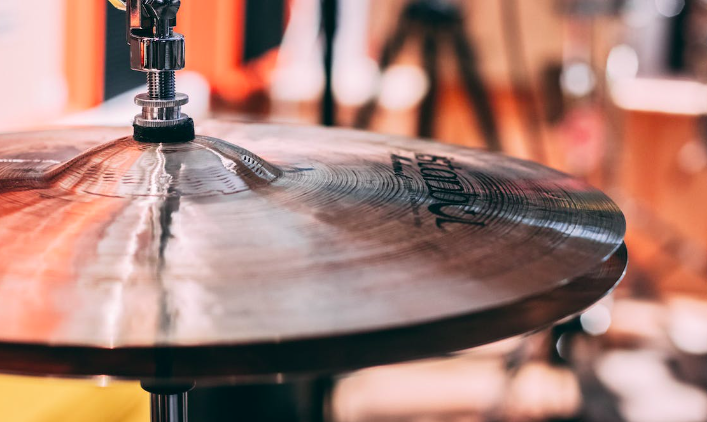
\includegraphics[width=4.16667in,height=3.03125in]{media/image1.png}

O efeito de sentido produzido pela charge é bem claro. Assinale
alternativa que apresenta tais efeitos de sentido:

\begin{enumerate}
\def\labelenumi{\alph{enumi})}
\item
  Ironia, humor e crítica
\item
  Informação, sensibilização e divulgação de conhecimento
\item
  Ironia, convencimento e formação de opinião
\item
  Crítica, sensibilização e divulgação de conhecimento
\end{enumerate}

Inferir, em textos multissemiótico, efeitos de humor, ironia e/ou
crítica

Bncc: EF69LP05

Inferir e justificar, em textos multissemióticos -- tirinhas, charges,
memes, gifs etc. --, o efeito de humor, ironia e/ou crítica pelo uso
ambíguo de palavras, expressões ou imagens ambíguas, de clichês, de
recursos iconográficos, de pontuação etc.

a) Correta. A ambiguidade se dá entre as palavras da faixa e a situação
da onça. O uso dos recursos verbais e não verbais produzem tais efeitos
de sentido

b) Incorreta. O efeito de sentido produzido pela charge não tem como
objetivo informar, ou divulgar conhecimentos, embora se possa considerar
a sensibilização como característica

c) Incorreta. Não há intenção de convencimento e formação de opinião
explícitos na charge

d) Incorreta. Não há intenção de divulgação de conhecimento, embora as
demais características podem decorrer da leitura deste gênero textual
multissemiótico

\textbf{Questão 8:}

A teórica Kirin Narayan questiona esse dualismo e foca na qualidade das
relações que mantemos com as pessoas que buscamos representar em nossos
textos. Nesse sentido, a autora propõe desconstruir a ideia de que os
interlocutores poderiam ser classificados como meros indivíduos para
declarações acerca de um \textbf{``outro generalizado}'', impulsionando
assim um entendimento desses sujeitos como portadores de
\textbf{``vozes, perspectivas e dilemas''} (1993, p. 672).

BOMFIM, Leonardo. Desafios e potencialidades do
``pesquisadornativo'':perspectivas etnográficas em um festival musical.
Disponível em:
\href{https://econtents.bc.unicamp.br/inpec/index.php/muspop/article/view/17627/12474}{{https://econtents.bc.unicamp.br/inpec/index.php/muspop/article/view/17627/12474}}.
Acesso em 24 de Abr. de 2023

Os termos destacados que aparecem entre aspas representam:

\begin{enumerate}
\def\labelenumi{\alph{enumi})}
\item
  as falas do autor sobre o tema
\item
  ideias que devem ser reforçadas
\item
  partes principais do argumento
\item
  citação direta das palavras da teórica Kirin Naryan
\end{enumerate}

Saeb:Analisar efeitos de sentido produzido pelo uso de formas de
apropriação textual (paráfrase, citação etc.)

a) Incorreta. O trecho não representa o pensamento do autor

b) Incorreta. O uso das aspas nesses casos não tem como função enfatizar

c) Incorreta. O trecho em destaque não tem como função enfatizar as
expressões

d) Correta. Os trechos em destaque aparecem entre aspas pois remetem a
falas da pesquisadora. Isso pode ser comprovado pela presença da
referência no final da frase.

\textbf{Questão 9:}

\textbf{Pedro Rezende: maior youtuber de games do país}

Falando sobre o jogo "Minecraft", Pedro Rezende se consolidou como o
maior YouTuber de games do Brasil ``A ideia inicial começou quando eu
precisava de ajuda para passar de uma fase em um jogo e procurei na
internet''.

A fala é de um dos maiores youtubers da atualidade no Brasil. O jovem
paranaense Pedro Rezende (19) mudou sua vida da água para o vinho depois
que abandonou a profissão de goleiro em um time de futebol na Itália
para seguir a carreira de youtuber de games por aqui.

https://auniao.pb.gov.br/noticias/caderno\_diversidade/geracao-de-youtubers-faz-sucesso-entre-os-jovens-do-pais\#:\textasciitilde:text=Figuras\%20como\%20K\%C3\%A9fera\%20Buchmann\%2C\%20Jout,jovens\%20e\%20adolescentes\%20do\%20pa\%C3\%ADs.

Com a expressão, `mudou sua vida da água para o vinho'' pode-se
compreender que o autor considera que:

\begin{enumerate}
\def\labelenumi{\alph{enumi})}
\item
  a vida do garoto não é fácil
\item
  que o garoto trocou água por vinho
\item
  que a vida do garoto continua a mesma
\item
  que a vida do garoto mudou drasticamente
\end{enumerate}

Saeb:Analisar o uso de figuras de linguagem como estratégia
argumentativa.

a) Incorreta. A expressão não se refere a esse aspceto

b) Incorreta. A expressão não pode ser tomada de forma literal

c) Incorreta. A expressão significa mudança

d) Correta. A expressão apresenta uma metáfora e representa uma grande
mudança

\textbf{Questão 10:}

Leia a manchete abaixo e responda:

\hypertarget{ariel-a-pequena-sereia-uxe9-opuxe7uxe3o-de-teatro-para-as-crianuxe7as-neste-final-de-semana}{%
\section{\texorpdfstring{\textbf{"Ariel, a Pequena Sereia" é opção de
teatro para as crianças neste final de
semana}}{"Ariel, a Pequena Sereia" é opção de teatro para as crianças neste final de semana}}\label{ariel-a-pequena-sereia-uxe9-opuxe7uxe3o-de-teatro-para-as-crianuxe7as-neste-final-de-semana}}

\hypertarget{espetuxe1culo-retorna-ao-teatro-barreto-juxfanior-neste-suxe1bado-22-e-domingo-23-uxe0s-16h30}{%
\subsection{Espetáculo retorna ao Teatro Barreto Júnior, neste sábado
(22) e domingo (23), às
16h30}\label{espetuxe1culo-retorna-ao-teatro-barreto-juxfanior-neste-suxe1bado-22-e-domingo-23-uxe0s-16h30}}

\href{https://www.folhape.com.br/cultura/ariel-a-pequena-sereia-e-opcao-de-teatro-para-as-criancas-neste/267280/.A}{{https://www.folhape.com.br/cultura/ariel-a-pequena-sereia-e-opcao-de-teatro-para-as-criancas-neste/267280/.A}}
ceso em 20 de Abr de 2023

O termo entre aspas indica:

\begin{enumerate}
\def\labelenumi{\alph{enumi})}
\item
  citação da fala de um entrevistado
\item
  citação do nome de uma obra
\item
  citação de uma gíria
\item
  pretende dar ênfase ao termo
\end{enumerate}

Analisar os efeitos de sentido decorrentes dos mecanismos de construção
de textos jornalísticos/midiáticos.

a) Incorreta. Não se trata de citação de fala

b) Correta. O trecho se refere a uma obra teatral

c) Incorreta. O trecho não se refere a uma gíria

d) Incorreta. O trecho não pretende dar ênfase ao termo

\textbf{Questão 11:}

\textbf{Texto 1:}

Às 14h, ocorreu o acidente. Um desmoronamento interno fez com que uma
enorme rocha se desprendesse da montanha e caísse sobre o túnel,
fechando completamente a ligação com a superfície. Dentro da mina,
ficaram 33 mineiros - 32 chilenos e 1 boliviano.

\href{https://www.bbc.com/portuguese/internacional-55926799}{{https://www.bbc.com/portuguese/internacional-55926799}}.
Acesso em 25 de Abr de 2023

\textbf{Texto 2:}

No dia 5 de agosto, um desmoronamento deixou 33 operários presos na mina
de San José, situada no deserto do Atacama, no Chile . Eles ficaram
incomunicáveis, a 700 metros de profundidade, durante 17 dias, até serem
descobertos pelas equipes de sondagem

\href{https://vestibular.uol.com.br/resumo-das-disciplinas/atualidades/mineiros-do-chile-o-resgate-que-emocionou-o-mundo.htm\#:~:text=Foram\%20constru\%C3\%ADdas\%20tr\%C3\%AAs\%20c\%C3\%A1psulas\%20de,todos\%20os\%20demais\%20foram\%20salvos}{{https://vestibular.uol.com.br/resumo-das-disciplinas/atualidades/mineiros-do-chile-o-resgate-que-emocionou-o-mundo.htm\#:\textasciitilde:text=Foram\%20constru\%C3\%ADdas\%20tr\%C3\%AAs\%20c\%C3\%A1psulas\%20de,todos\%20os\%20demais\%20foram\%20salvos}}..
Acesso em 25 de Abr de 2023

Com base na informações dos dois textos é correto afirmar que:

\begin{enumerate}
\def\labelenumi{\alph{enumi})}
\item
  O acidente ocorreu às 14 horas
\item
  O acidente deixou 33 operários presos
\item
  Os mineiros ficaram presos por 17 dias
\item
  O acidente atingiu 32 chilenos e 1 boliviano
\end{enumerate}

Avaliar a fidedignidade de informações sobre um mesmo fato divulgado em
diferentes veículos e mídias.

\begin{enumerate}
\def\labelenumi{\alph{enumi})}
\item
  Incorreta. A informação aparece apenas no texto 1
\item
  Correta. A informação aparece nos dois textos.
\item
  Incorreta. Apenas o texto 2 traz essa informação
\item
  Incorreta.Apenas o texto 1 traz essa informação
\end{enumerate}

\textbf{Questão 12:}

Nordeste poderia crescer mais que o Brasil até 2030

Combinar aumento da produtividade com redução das desigualdades seria a
melhor alternativa para elevar o PIB per capita na região

\href{https://www.ipea.gov.br/portal/categorias/45-todas-as-noticias/noticias/9506-nordeste-poderia-crescer-mais-que-o-brasil-ate-2030?highlight=WyJub3JkZXN0ZSIsIm5vcmRlc3RlJy4iXQ==}{{https://www.ipea.gov.br/portal/categorias/45-todas-as-noticias/noticias/9506-nordeste-poderia-crescer-mais-que-o-brasil-ate-2030?highlight=WyJub3JkZXN0ZSIsIm5vcmRlc3RlJy4iXQ==}}
Acesso em 25 de Abr de 2023

Leia o texto e assinale a alternativa correta:

\begin{enumerate}
\def\labelenumi{\alph{enumi})}
\item
  O texto afirma que o Nordeste vai crescer mais que o Brasil até 2030 e
  aumentar a produtividade para diminuir a desigualdade
\item
  O texto coloca como condição o aumento de produtividade e redução da
  desigualdade para que haja maior crescimento do Nordeste em relação ao
  Brasil
\item
  O texto afirma que a diminuição da desigualdade na região Nordeste
  ocorreu e vai elevar o PIB na região
\item
  O texto afirma que a elevação do PIB na região é consequência de seu
  crescimento maior em relação ao Brasil
\end{enumerate}

Identificar os recursos de modalização em textos diversos.

a) Incorreta. O texto não afirma o crescimento da região,pois utiliza o
verbo no futuro do pretérito

b) Correta. O uso do verbo no futuro do pretérito indica uma condição
para que a afirmação se consolide

c) Incorreta. O texto não afirma que houve a diminuição destes
problemas, mas que através disso, poderia crescer

d) Incorreta. O texto não afirma que teria ocorrido o aumento do PIB,
apenas condiciona este aumento à diminuição da desigualdades

\textbf{Questão 13:}

Aquiles, com a ameaça de perder o seu prêmio nos saques, entre os quais
estava uma linda moça, Briseida, \textbf{pela qual estava apaixonado,}
respondeu:

--Homem sem vergonha! Eu vim a Tróia guerrear os troianos, mas não tenho
nada contra eles.

ROCHA, R. Ilíada. São Paulo: Moderna, 2010. p.16.

No trecho em destaque, o uso do aposto indica que:

\begin{enumerate}
\def\labelenumi{\alph{enumi})}
\item
  Havia alguém apaixonado por Aquiles
\item
  Briseida estava apaixonada por um troiano
\item
  Os troianos estavam apaixonados por Briseida
\item
  Aquiles estava apaixonado por Briseida
\end{enumerate}

Analisar os processos de referenciação lexical e pronominal.

\begin{enumerate}
\def\labelenumi{\alph{enumi})}
\item
  Incorreta. O trecho não indica que o sentimento seja por Aquiles
\item
  Incorreta. O trecho não se refere aos sentimentos de Briseida
\item
  Incorreta. Os sentimentos dos troianos não aparecem no trecho
\item
  Correta. A função do termo aparece como referenciação pronominal e se
  refere aos sentimentos de Aquiles por Briseida
\end{enumerate}

\textbf{Questão 14:}

A vacina salva vidas. Doenças que causavam milhares de vítimas no
passado, como varíola e poliomielite, foram erradicadas. Outras doenças
transmissíveis também deixaram de ser problema de saúde pública porque
foram eliminadas no Brasil e nas Américas, como o sarampo, rubéola e
rubéola congênita.

Qual das seguintes opções melhor descreve a estratégia argumentativa
utilizada para enfatizar a importância da vacinação?

\begin{enumerate}
\def\labelenumi{\alph{enumi})}
\item
  Emoção
\item
  Generalização
\item
  Lógica
\item
  Autoridade
\end{enumerate}

Avaliar a eficácia das estratégias argumentativas em textos de
diferentes gêneros.

a) Incorreta.O autor não apela diretamente para as emoções do leitor,
mas sim para argumentos lógicos e fatos concretos.

b) Incorreta. O autor apresenta exemplos concretos de doenças
erradicadas e reduzidas graças à vacinação, e não faz generalizações
para enfatizar a importância da vacinação.

c) Correta. O autor usa uma abordagem lógica para argumentar a favor da
vacinação, apresentando exemplos de doenças erradicadas e reduzidas
graças à vacinação, tentando provar a vacinação como estratégia mais
eficaz para prevenir doenças e salvar vidas.

d) Incorreta. O autor não se apoia em autoridades ou especialistas para
argumentar a favor da vacinação, mas sim em fatos e exemplos concretos.

\textbf{Questão 15:}

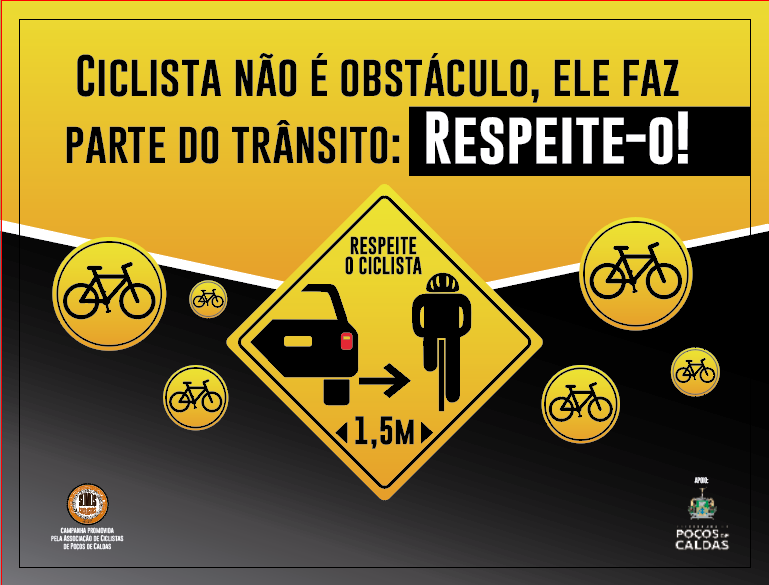
\includegraphics[width=5.90551in,height=3.18056in]{media/image2.png}

\href{https://www.tre-sp.jus.br/comunicacao/noticias/2022/Junho/campanha-201ctamo-junto201d-do-tre-sp-quer-incentivar-voto-consciente-dos-jovens}{{https://www.tre-sp.jus.br/comunicacao/noticias/2022/Junho/campanha-201ctamo-junto201d-do-tre-sp-quer-incentivar-voto-consciente-dos-jovens}}
acesso em 20 de Abr de 2023

Acima vemos um exemplo de campanha incentivando a votação. Ao analisar
as escolhas de linguagem utilizadas podemos afirmar que:

a) a campanha se dirige ao público idoso

b) a campanha se dirige ao público infantil

c) a campanha se dirige a mulheres

d) a campanha se dirige ao público jovem

Avaliar a adequação das variedades linguísticas em contextos de uso

a) Incorreta. O uso de recursos utilizados em redes sociais, tais como
símbolos e siglas não é o mais indicado ao público idoso

b) Incorreta. O uso de gírias, símbolos e siglas de internet não são os
mais eficazes para o público infantil

c) Incorreta. Não há nada na imagem que remeta ao público feminino

d) Correta. O uso de gírias, siglas e símbolos utilizados no meio
digital pode ser um recurso eficaz para atingir os jovens.

\textbf{Simulado 3}

\textbf{Questão 1:}

\textbf{Alimentos que prejudicam o meio ambiente são também os piores à
saúde}

Comer cereais, frutas, verduras, batatas e azeite de oliva protege o
planeta e previne doenças

Aproximadamente 60\% dos fatores de risco responsáveis por todas as
doenças são o resultado de uma dieta de má qualidade. Esse fato está
ligado à saúde do planeta. Um estudo publicado na revista PNAS demonstra
que os alimentos mais prejudiciais ao ser humano também o são para a
Terra.

Os pesquisadores analisaram 15 alimentos que fazem parte da dieta diária
ocidental. Ligaram a maneira como são produzidos (a água que se gasta, a
superfície implicada e os produtos químicos utilizados, entre outros)
aos resultados de estudos anteriores sobre o impacto desses mesmos
alimentos sobre a saúde. E tudo se encaixava. As frutas, verduras, a
batata, o azeite de oliva, os legumes, as frutas secas e os cereais são
os alimentos mais saudáveis e que, além disso, têm impacto mínimo sobre
o planeta.

A carne vermelha processada e não processada, por outro lado, é um
produto que deveria sair da lista de compras.

O peixe é um dilema. É uma opção saudável, como a maioria das pessoas
sabe, mas tem uma pegada ambiental maior, ao lado do frango e dos
laticínios, do que as dietas baseadas em vegetais, de acordo com os
resultados do estudo. Basulto afirma que um produto é benéfico quando
impede o consumidor de comer alimentos mais prejudiciais para sua saúde.
``Se o cliente come peixe e não consome carne vermelha, portanto, é bom
para ele e para o planeta'', acrescenta.

Disponível em
:\textless{}\href{https://brasil.elpais.com/brasil/2019/10/29/ciencia/1572344750_688431.html\#?rel=mas}{{https://brasil.elpais.com/brasil/2019/10/29/ciencia/1572344750\_688431.html\#?rel=mas}}\textgreater{}
. Acesso em 7 de abri 2023.

Segundo a reportagem, assinale a alternativa que contém os alimentos
mais saudáveis e que menos impactam o planeta:

\begin{enumerate}
\def\labelenumi{\alph{enumi})}
\item
  cereais, ovos, legumes
\item
  frutas, verduras, cereais
\item
  frutas, verduras, peixe
\item
  frutas secas, azeite, carnes
\end{enumerate}

Saeb:Identificar teses, opiniões, posicionamentos explícitos e
argumentos em textos.

a) Incorreta. A reportagem não cita os ovos.

b)Correta. Estes estão entre os alimentos mais saudáveis e de menor
impacto junto ao azeite e frutas secas

c) Incorreta. O peixe tem grande impacto, porém menor do que o consumo
de carnes vermelhas

d) Incorreta. As carnes, segundo a reportagem, deveriam ser retiradas
das dietas

\textbf{Questão 2:}

No caso, a quantidade de comida industrializada ingerida parece
influenciar no aparecimento de doenças e na quantidade de mortes
prematuras. Esses estudos, no entanto, não conseguem demonstrar qual
seria o mecanismo por trás dessa aparente correlação.

A geriatra Claudia Suemoto, da Faculdade de Medicina da USP, que
coordenou o estudo do Elsa sobre ultraprocessados e desempenho
cognitivo, espera superar essa limitação em breve. Serão feitas imagens
do cérebro de voluntários para ver se o alto consumo de ultraprocessados
pode causar eventos isquêmicos ou pequenos derrames cerebrais, que, ao
longo do tempo, poderiam comprometer as funções cognitivas. ``Dessa
forma, poderemos investigar possíveis mecanismos que expliquem a
associação do ponto de vista estrutural'', conta Suemoto.

Segundo o texto, a limitação a ser superada pela pesquisa é:

\begin{enumerate}
\def\labelenumi{\alph{enumi})}
\item
  diminuir a quantidade de ingestão de ultraprocessados e melhorar o
  desempenho cognitivo
\item
  demonstrar o mecanismo por trás da relação entre o consumo de
  ultraprocessados e as mortes prematuras
\item
  conseguir imagens do cérebro de voluntários que sofreram derrame
  cerebral
\item
  estudar as funções cognitivas e os eventos isquêmicos de quem sofreu
  derrame cerebral
\end{enumerate}

Identificar elementos constitutivos de gêneros de divulgação científica.

a) Incorreta. O estudo não visa diminuir o consumo de ultraprocessados

b) Correta. A limitação apresentada em outros estudos é demonstrar quais
os mecanismos do alto consumo de ultraprocessados ocorrem no cérebro e
que podem levar a derrames

c) Incorreta. O texto não cita que esta seja uma limitação

d) Incorreta. O texto não afirma que este estudo seja uma limitação

\textbf{Questão 3:}

Título I

Das Disposições Preliminares

Art. 1º Esta Lei dispõe sobre a proteção integral à criança e ao
adolescente.

Art. 2º Considera-se criança, para os efeitos desta Lei, a pessoa até
doze anos de idade incompletos, e adolescente aquela entre doze e
dezoito anos de idade.

Parágrafo único. Nos casos expressos em lei, aplica-se excepcionalmente
este Estatuto às pessoas entre dezoito e vinte e um anos de idade.

\href{https://www.planalto.gov.br/ccivil_03/leis/l8069.htm}{{https://www.planalto.gov.br/ccivil\_03/leis/l8069.htm}}.
Acesso em 25 de Abr de 2023

Estão presentes no texto acima e são características de textos legais ou
jurídicos:

\begin{enumerate}
\def\labelenumi{\alph{enumi})}
\item
  Linguagem genérica e impessoal e organizado em títulos, capítulos e
  sessões.
\item
  Uso de linguagem informal e composto por parágrafos e estrofes
\item
  Linguagem rebuscada e composto por títulos e subtítulos
\item
  Pode ser escrito em primeira pessoa e organizado de forma livre
\end{enumerate}

Saeb: Identificar formas de organização de textos normativos, legais
e/ou reivindicatórios.

Bncc: EF69LP20 Identificar, tendo em vista o contexto de produção, a
forma de organização dos textos normativos e legais, a lógica de
hierarquização de seus itens e subitens e suas partes: parte inicial
(título -- nome e data -- e ementa), blocos de artigos (parte, livro,
capítulo, seção, subseção), artigos (caput e parágrafos e incisos) e
parte final (disposições pertinentes à sua implementação) e analisar
efeitos de sentido causados pelo uso de vocabulário técnico, pelo uso do
imperativo, de palavras e expressões que indicam circunstâncias, como
advérbios e locuções adverbiais, de palavras que indicam generalidade,
como alguns pronomes indefinidos, de forma a poder compreender o caráter
imperativo, coercitivo e generalista das leis e de outras formas de
regulamentação.

\textbf{Questão 4:}

\textbf{Faciap promove encontros para jovens empreendedores em Curitiba}

Entre quinta (25) e sexta-feira (26) acontecem dois eventos promovidos
pelos integrantes da ala jovem da Federação das Associações Comerciais e
Empresariais do Paraná (Faciap).

A Assembleia Geral Ordinária (AGO) da Confederação Nacional de Jovens
Empresários (Conaje), que começa nesta quinta-feira (25) é um evento
nacional e vai reunir jovens empreendedores de todo o Brasil. Já na
sexta-feira (26) acontece o Encontro Paranaense de Jovens
Empreendedores.

\href{https://cbncuritiba.com.br/materias/faciap-promove-encontros-para-jovens-empreendedores-em-curitiba/}{{https://cbncuritiba.com.br/materias/faciap-promove-encontros-para-jovens-empreendedores-em-curitiba/}}.
Acesso em 25 de Abr de 2023.

Considerando os elementos constitutivos dos textos jornalísticos, a
informação sobre a cidade onde ocorre o evento é denominada:

\begin{enumerate}
\def\labelenumi{\alph{enumi})}
\item
  Corpo da notícia
\item
  Lide
\item
  Título auxiliar
\item
  Manchete
\end{enumerate}

Identificar elementos constitutivos de textos pertencentes ao domínio

jornalístico/midiático.

a) Incorreta. O corpo da notícia aparece depois da manchete e do lide.

b) Incorreta. O lide ou \emph{lead,} neste caso, não apresenta o nome da
cidade

c) Incorreta. O exemplo não contém título auxiliar

d) Correta. A informação aparece muito claramente já na manchete ou
título da notícia

\textbf{Questão 5:}

O Guardador de Rebanhos

Alberto Caeiro

Mas a minha tristeza é sossego

Porque é natural e justa

E é o que deve estar na alma

Quando já pensa que existe

E as mãos colhem flores sem ela dar por isso.

\href{http://www.dominiopublico.gov.br/download/texto/pe000001.pdf}{{http://www.dominiopublico.gov.br/download/texto/pe000001.pdf}}.
Acesso em 26 de Abr. de 2023\\
Nesta estrofe do poema, a opinião do autor sobre o sossego de sua
tristeza está expressa em:

\begin{enumerate}
\def\labelenumi{\alph{enumi})}
\item
  Mas a minha tristeza é sossego
\item
  \ldots é o que deve estar na alma
\item
  E as mão colhem flores
\item
  Porque é natural e justa
\end{enumerate}

Inferir informações implícitas em distintos textos

a) Incorreta. Este trecho contém a afirmação de que a tristeza é sossego

b)Incorreta. este trecho complementa a ideia mas não é a opinião central

c) Incorreta. O trecho apenas ilustra a opinião

d) Correta. O uso do porque expressa uma explicação sobre a afirmação
anterior sobre a tristeza

\textbf{Questão 6:}

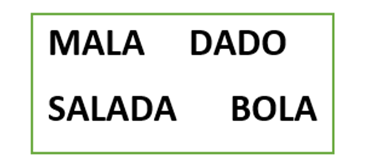
\includegraphics[width=5.90551in,height=1.70833in]{media/image3.png}

\href{https://tirasarmandinho.tumblr.com/}{{https://tirasarmandinho.tumblr.com/}}.
Acesso em 26 de Abr de 2023

A ironia no quadrinho está expressa em:

\begin{enumerate}
\def\labelenumi{\alph{enumi})}
\item
  Estar sem emprego me deixa triste
\item
  a cada dia há mais pessoas como você
\item
  Não fique triste\ldots{}
\item
  O senhor não está sozinho
\end{enumerate}

Inferir, em textos multissemiótico, efeitos de humor, ironia e/ou
crítica.

Bncc: EF69LP05 Inferir e justificar, em textos multissemióticos --
tirinhas, charges, memes, gifs etc. --, o efeito de humor, ironia e/ou
crítica pelo uso ambíguo de palavras, expressões ou imagens ambíguas, de
clichês, de recursos iconográficos, de pontuação etc.

a) Incorreta. O primeiro quadro expressa o sentimento do pai

b) Incorreta. Esta frase apenas complementa a ironia

c) Incorreta. O trecho introduz a fala irônica de Armandinho

d) Correta. A ironia se encontra neste trecho, pois Armandinho dá a
entender que pelo fato de haver mais pessoas na mesma situação o pai não
deveria se sentir triste

\textbf{Questão 7}

\textbf{Exemplo 1:}

Câncer de mama

É o tipo de câncer mais frequente na mulher brasileira. Nesta doença,
ocorre um desenvolvimento anormal das células da mama, que
multiplicam-se repetidamente até formarem um tumor maligno.

Como descobrir a doença mais cedo?

Toda mulher com 40 anos ou mais de idade deve procurar um ambulatório,
centro ou posto de saúde para realizar o exame clínico das mamas
anualmente, além disso, toda mulher, entre 50 e 69 anos deve fazer pelo
menos uma mamografia a cada dois anos. O serviço de saúde deve ser
procurado mesmo que não tenha sintomas!

O que é o exame clínico das mamas?

É o exame das mamas realizado por médico ou enfermeiro treinado para
essa atividade. Neste exame poderão ser identificadas alterações nas
mesmas. Se for necessário, será indicado um exame mais específico, como
a mamografia.

O auto-exame previne a doença?

O exame das mamas realizado pela própria mulher, apalpando os seios,
ajuda no conhecimento do próprio corpo, entretanto, esse exame não
substitui o exame clínico das mamas realizado por um profissional de
saúde treinado. Caso a mulher observe alguma alteração deve procurar
imediatamente o serviço de saúde mais próximo de sua residência. Mesmo
que não encontre nenhuma alteração no auto-exame, as mamas devem ser
examinadas uma vez por ano por um profissional de saúde!

Fonte: Instituto Nacional de Câncer. Câncer de mama

\href{https://bvsms.saude.gov.br/cancer-de-mama/}{{https://bvsms.saude.gov.br/cancer-de-mama/}}.
Acesso em 26 de Abr de 2023

\textbf{Exemplo 2:}

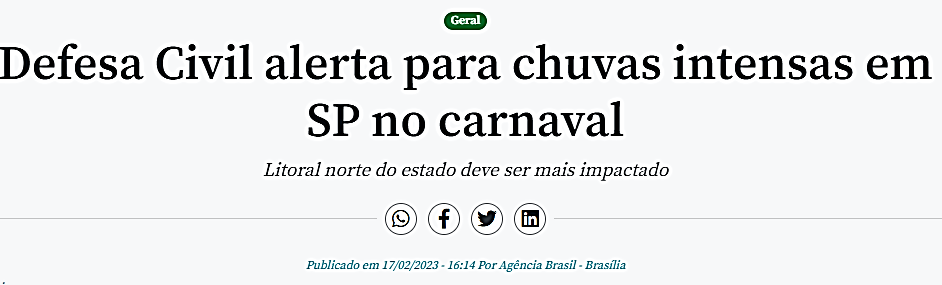
\includegraphics[width=3.73839in,height=3.73839in]{media/image4.png}

\href{https://www.gov.br/arquivonacional/pt-br/canais_atendimento/imprensa/copy_of_noticias/cancer-de-mama-e-hora-de-falar-sobre-isso}{{https://www.gov.br/arquivonacional/pt-br/canais\_atendimento/imprensa/copy\_of\_noticias/cancer-de-mama-e-hora-de-falar-sobre-isso}}.
Acesso em 26 de abr de 2023

Os dois exemplos trazem informações sobre o câncer de mama e os exames
necessários para detectar a doença. Nos dois casos, o que faz com que as
informações sejam confiáveis é a presença de:

\begin{enumerate}
\def\labelenumi{\alph{enumi})}
\item
  textos explicativos
\item
  figuras e textos
\item
  citação de fontes oficiais
\item
  linguagem clara
\end{enumerate}

Saeb:Avaliar a fidedignidade de informações sobre um mesmo fato
divulgado em diferentes veículos e mídias.

a) Incorreta. Embora os textos sejam bastante explicativos, este não é
um critério de confiabilidade

b) Incorreta. As figuras e textos só aparecem no Exemplo 2 e não podem
ser considerados recursos para avaliar a confiabilidade das informações

c) Correta. Em ambos os casos a fonte das informações é o INCA, órgão
oficial que trata das questões relativas ao câncer de mama e demais
formas da doença

d) Incorreta. Embora a linguagem utilizada seja clara, este não é um
critério de confiabilidade

\textbf{Questão 8:}

O que a ciência diz sobre os remédios naturais para dormir

Se você tomar um chazinho à base de ervas ou borrifar o quarto com
aromas agradáveis... será que vai conseguir dormir como um bebê?

O sono raramente é mais desejado do que quando não conseguimos dormir.

E há uma grande variedade de remédios caseiros que prometem nos ajudar a
pegar no sono sem recorrer a produtos farmacêuticos.

\href{https://g1.globo.com/saude/noticia/2023/04/26/o-que-a-ciencia-diz-sobre-os-remedios-naturais-para-dormir.ghtml}{{https://g1.globo.com/saude/noticia/2023/04/26/o-que-a-ciencia-diz-sobre-os-remedios-naturais-para-dormir.ghtml}}.
Acesso em 26 de Abr de 2023

A expressão raramente, para se referir ao desejo de dormir expressa:

\begin{enumerate}
\def\labelenumi{\alph{enumi})}
\item
  que dificilmente pode-se desejar sentir sono, exceto em casos de
  insônia
\item
  que na maioria das vezes o sono é desejado em qualquer ocasião
\item
  que sempre sentimos sono quando precisamos dormir
\item
  que só sentimos sono quando não desejamos dormir
\end{enumerate}

Analisar os efeitos de sentido produzidos pelo uso de modalizadores em
textos diversos.

a) Correta. A frase expressa que o sono é muito desejado quando se tem
insônia, deixando implícita a ideia de que não desejamos sentir sono em
outras ocasiões

b) Incorreta. O advérbio raramente deixa implícita a ideia de que
dificilmente o sono será desejado em outras ocasiões

c) Incorreta. Na expressão a ideia é contrária a esta

d) Incorreta. De acordo com a afirmação não se pode inferir essa
afirmação

\textbf{Questão 9}

\textbf{Poeminha Maçante}

\textbf{- Por que não ser também um chato?}

(...)Mas de repente percebi

Sem ser doutor

Que a chatice é a única doença

que não dói no portador

E resolvi ser chato. (...)

Fernandes, Millor. Circo de palavras: histórias, poemas, pensamentos.
São Paulo: Ática, 2007. p.63

Segundo o poema, qual o motivo do autor ter escolhido ser chato:

\begin{enumerate}
\def\labelenumi{\alph{enumi})}
\item
  Por ser uma doença
\item
  Porque ser chato não dói
\item
  Porque ele queria ser doutor
\item
  Porque percebeu-se chato de repente
\end{enumerate}

Avaliar a eficácia das estratégias argumentativas em textos de
diferentes gêneros.

a) Incorreta. Embora ele afirme que a chatice seja uma doença, não é
este o motivo

b) Correta. A autor diz que sendo a única doença que não dói, resolveu
ser chato

c) Incorreta. Ele afirma que não precisa ser doutor para saber que a
chatice é uma doença

d) Incorreta. Não há elementos no texto que levem a esta afirmação

\textbf{Questão 10}

O casamento fez-se onze meses depois, e foi a mais bela festa das
relações dos noivos. Amigas de Clara, \textbf{menos por amizade que por
inveja}, tentaram arredá-la do passo que ia dar. Não negavam a gentileza
do noivo, nem o amor que lhe tinha, nem ainda algumas virtudes; diziam
que era dado em demasia a patuscadas.

O trecho em destaque expressa:

\begin{enumerate}
\def\labelenumi{\alph{enumi})}
\item
  que as amigas de Clara tentaram impedir o casamento pela amizade que
  tinham por ela
\item
  que as amigas de Clara consentiam com o casamento
\item
  que as amigas de clara não nutriam qualquer amizade verdadeira por ela
\item
  que as amigas de Clara tentaram impedir o casamento por sentirem
  inveja, embora houvesse amizade entre elas
\end{enumerate}

Analisar os processos de referenciação lexical e pronominal.

a) Incorreta. A ideia transmitida é de que as amigas tentaram impedir o
casamento não apenas por amizade

b) Incorreta. As amigas de Clara não aprovavam o casamento

c) Incorreta. Não é possível inferir essa afirmação a partir do trecho

d) Correta. O uso da expressão menos por\ldots que por\ldots{} indica
que havia sentimento de amizade, embora ele não tenha sido o motivo
principal das amigas se oporem ao casamento

\textbf{Questão 11}

I. \textbf{Já que} o vento soprava muito forte, decidiram não sair
naquela noite.

II. Eu não consegui ir ao escritório \textbf{porque} estava muito doente

III. Os jovens terão suas necessidades ouvidas, \textbf{exceto} se se
afastarem dos responsáveis.

IV. Estava triste, \textbf{mas} não chorou.

Assinale a alternativa que indica corretamente as relações de sentido
produzidas pelos conectivos em destaque:

a) causa, causa, condição, oposição.

b) comparação, condição, finalidade, oposição.

c) causa, oposição, condição, finalidade

d) finalidade, comparação, tempo, causa.

Analisar os mecanismos que contribuem para a progressão textual.

a) Correta. já que\ldots foi a causa de não terem saído, estar doente
foi a causa de não ir ao escritório; a condição para o jovens serem
ouvidos é que tenham relação de proximidade com os responsáveis; apesar
de estar triste, não chorar, indica oposição

b) Incorreta. Exemplo I não apresenta comparação; II não apresenta
condição; III não apresenta finalidade.

c) Incorreta. II não apresenta oposição; IV não apresenta finalidade.

d) Incorreta. I não apresenta finalidade; II não apresenta comparação;
II não representa tempo; IV não representa causa.

\textbf{Questão 12}

\hypertarget{agrotuxf3xicos-no-brasil-o-veneno-ainda-estuxe1-na-mesa}{%
\section{Agrotóxicos no Brasil: O veneno ainda está na
mesa}\label{agrotuxf3xicos-no-brasil-o-veneno-ainda-estuxe1-na-mesa}}

Em relação ao consumo de agrotóxicos no Brasil, hoje paira uma grande
incerteza sobre os números exatos. No ano de 2015, só foram divulgados
os valores em dólares dos ganhos da indústria. Neste sentido, houve uma
forte queda, de 21\%, em relação a 2014. No entanto, se considerarmos a
variação do câmbio, vemos que na verdade o faturamento em reais subiu de
R\$28 para R\$32 bilhões. Como uma boa parte do custo dos agrotóxicos é
importada, não é possível saber se aumentou ou diminuiu a quantidade de
agrotóxicos em 2015.

\href{https://www.brasildefato.com.br/2016/11/23/agrotoxicos-no-brasil-o-veneno-ainda-esta-na-mesa}{{https://www.brasildefato.com.br/2016/11/23/agrotoxicos-no-brasil-o-veneno-ainda-esta-na-mesa}}.
Acesso em 26 de Abr de 2023.

Assinale a alternativa que contém a figura de linguagem correta e o
trecho em que aparece:

\begin{enumerate}
\def\labelenumi{\alph{enumi})}
\item
  Hipérbole. Agrotóxicos do Brasil
\item
  Metáfora.(...) hoje paira uma grande incerteza sobre os números exatos
\item
  Metonímia. O veneno ainda está na mesa
\item
  Hipérbole. Neste sentido, houve uma forte queda, de 21\%
\end{enumerate}

Analisar o uso de figuras de linguagem como estratégia argumentativa.

a) Incorreta\textbf{.} O trecho não apresenta figura de linguagem

b) Incorreta. O trecho não apresenta figura de linguagem

c) Correta. O trecho apresenta metonímia quando usa o termo mesa para se
referir a alimentação

d) Incorreta. O trecho não apresenta figura de linguagem

\textbf{Questão 13}

A viagem era curta, \textbf{e os versos pode ser que não fossem
inteiramente maus.} Sucedeu, porém, que, como eu estava cansado, fechei
os olhos três ou quatro vezes; tanto bastou para que ele interrompesse a
leitura e metesse os versos no bolso.

A escolha dos verbos no trecho em destaque dá a entender que:

\begin{enumerate}
\def\labelenumi{\alph{enumi})}
\item
  O autor considerava os versos ruins e interrompeu a leitura
\item
  O autor considerava os versos bons mas que a viagem era curta
\item
  O autor considera que os versos o deixaram cansado
\item
  O autor considera que os versos não eram nem bons nem ruins, mas que
  ele estava cansado
\end{enumerate}

Analisar os efeitos de sentido dos tempos, modos e/ou vozes verbais com
base no gênero textual e na intenção comunicativa.

a) Incorreta. O autor não deixa claro que considerava os versos ruins, o
que pode ser comprovado pela escolha dos verbos e modos verbais

b) Incorreta. O autor não deixa claro que considera os versos bons, o
que pode ser comprovado pela escolha dos verbos e modos verbais

c) Incorreta. O autor não atribui seu cansaço aos versos

d) Correta. O uso dos tempos e modos verbais dão a entender que
independente da qualidade dos versos e da duração da viagem, ele fechou
os olhos porque estava cansado.

\textbf{Questão 14:}

\hypertarget{os-cosplays-mais-irados-de-2021}{%
\section{\texorpdfstring{\textbf{Os cosplays mais irados de
2021}}{Os cosplays mais irados de 2021}}\label{os-cosplays-mais-irados-de-2021}}

\hypertarget{apesar-da-pandemia-a-criatividade-na-cultura-pop-nuxe3o-parou-por-isso-vamos-ver-os-cosplays-que-mais-se-destacaram-em-2021-atuxe9-agora}{%
\subsection{Apesar da pandemia, a criatividade na cultura pop não parou,
por isso, vamos ver os cosplays que mais se destacaram em 2021 até
agora!}\label{apesar-da-pandemia-a-criatividade-na-cultura-pop-nuxe3o-parou-por-isso-vamos-ver-os-cosplays-que-mais-se-destacaram-em-2021-atuxe9-agora}}

\href{https://www.terra.com.br/gameon/geek/os-cosplays-mais-irados-de-2021,b409f1697bb7db34500d0614340e6423966k7p1p.html}{{https://www.terra.com.br/gameon/geek/os-cosplays-mais-irados-de-2021,b409f1697bb7db34500d0614340e6423966k7p1p.html}}.
Acesso em 26 de Abr. de 2023

No exemplo acima, vemos algumas variações linguísticas. Assinale a
alternativa que contém o termo e o tipo de variação presentes no texto:

\begin{enumerate}
\def\labelenumi{\alph{enumi})}
\item
  cosplays/estrangeirismo; irado/gíria
\item
  cultura pop/ gíria; cosplay/estrangeirismo
\item
  irados/ regionalismo; cosplay/gíria
\item
  irados/geográfica; cultura pop/gíria
\end{enumerate}

Analisar as variedades linguísticas em textos

a) Correta. O termo cosplay vem do inglês mas foi incorporado pela
cultura pop e o termo irado está sendo usado como gíria e não com o
sentido literal

b) Incorreta. Os dois termos são estrangeirismos

c) Incorreta. Irado aparece como gíria e cosplay é estrangeirismo

d) Incorreta. Irado está sendo usado como gíria e a palavra pop é um
estrangeirismo

\textbf{Questão 15:}

OS ``CAUSOS'' DE JOSELI DIAS

O ofício de jornalista de Joseli Dias deu-lhe a agilidade de lidar com
as palavras. As narrativas das lendas e dos ``causos'' desta região,
reunidas no livro Mitos e Lendas do Amapá, se constituem em um trabalho
de suma importância para todos nós, que valorizamos os elementos mais
puros e autênticos da nossa cultura popular.

Dias, Joseli. Mitos e lendas no Amapá . 4. ed.Brasília : Senado

Federal, Conselho Editorial, 2020.

Disponível em:
\href{https://www2.senado.leg.br/bdsf/bitstream/handle/id/576836/Mitos_lendas_Amapa.pdf}{{https://www2.senado.leg.br/bdsf/bitstream/handle/id/576836/Mitos\_lendas\_Amapa.pdf}}.
Acesso em 26 de Abr. de 2023

O uso do termo ``causos'' se justifica pois:

\begin{enumerate}
\def\labelenumi{\alph{enumi})}
\item
  o texto que se apresenta exige linguagem formal
\item
  o autor não teve acesso à escola
\item
  o termo se refere a uma gíria
\item
  se trata de um regionalismo usado na cultura popular
\end{enumerate}

Avaliar a adequação das variedades linguísticas em contextos de uso

a) Incorreta. O texto não apresenta linguagem formal

b) Incorreta. O uso de variações linguísticas não deve ser considerado
um erro, correndo o risco de incorrer em preconceito linguístico

c) Incorreta. O termo não se refere a uma gíria e sim a uma variação
linguística de cunho regional

d) Correta. Por se tratar de um gênero da tradição popular, o termo pode
ser utilizado como variação linguística.

\textbf{Simulado 4}

\textbf{Questão 1:}

\textbf{França limitará o aumento do preço da eletricidade até 2025}

Recuperação da atividade econômica após a pandemia do coronavírus
provocou uma alta nos preços da energia na Europa

A França vai prolongar até 2025 os subsídios adotados em outubro de 2021
para limitar o aumento do preço da eletricidade, em um contexto de
preocupação com a perda de poder de compra, anunciou o governo nesta
sexta-feira (21).

Le Maire alertou, por outro lado, que encerrará este ano o programa para
limitar o aumento dos preços do gás, já que estes "voltaram ao nível
anterior à crise, de 50 euros por megawatt-hora".

A recuperação da atividade econômica após a pandemia do coronavírus
provocou uma alta nos preços da energia na Europa no final de 2021, que
disparou meses depois com o início da invasão russa à Ucrânia.

https://www.folhape.com.br/noticias/franca-limitara-o-aumento-do-preco-da-eletricidade-ate-2025/267267/
. Acesso em Abr de 2023

Segundo a matéria a justificativa para o aumento do preço da
eletricidade se deve:

\begin{enumerate}
\def\labelenumi{\alph{enumi})}
\item
  à recuperação econômica pós pandemia e falta economia dos franceses
\item
  ao programa do do governo que se encerra
\item
  à recuperação da atividade econômica e a guerra na Ucrânia
\item
  à preocupação com o poder de compra dos franceses
\end{enumerate}

Identificar teses, opiniões, posicionamentos explícitos e argumentos em
textos.

a) Incorreta. O texto não fala da atitude dos consumidores

b) Incorreta. Embora o texto cite a interrupção do programa, não é um
fator que tenha interferido no aumento

c) Correta. Segundo o texto estes são os principais fatores que levaram
ao aumento dos preços da energia na Europa

d) Incorreta. O texto trata do poder de compra dos franceses como uma
preocupação mas não trata a questão como fator para o aumento da energia

\textbf{Questão 2:}

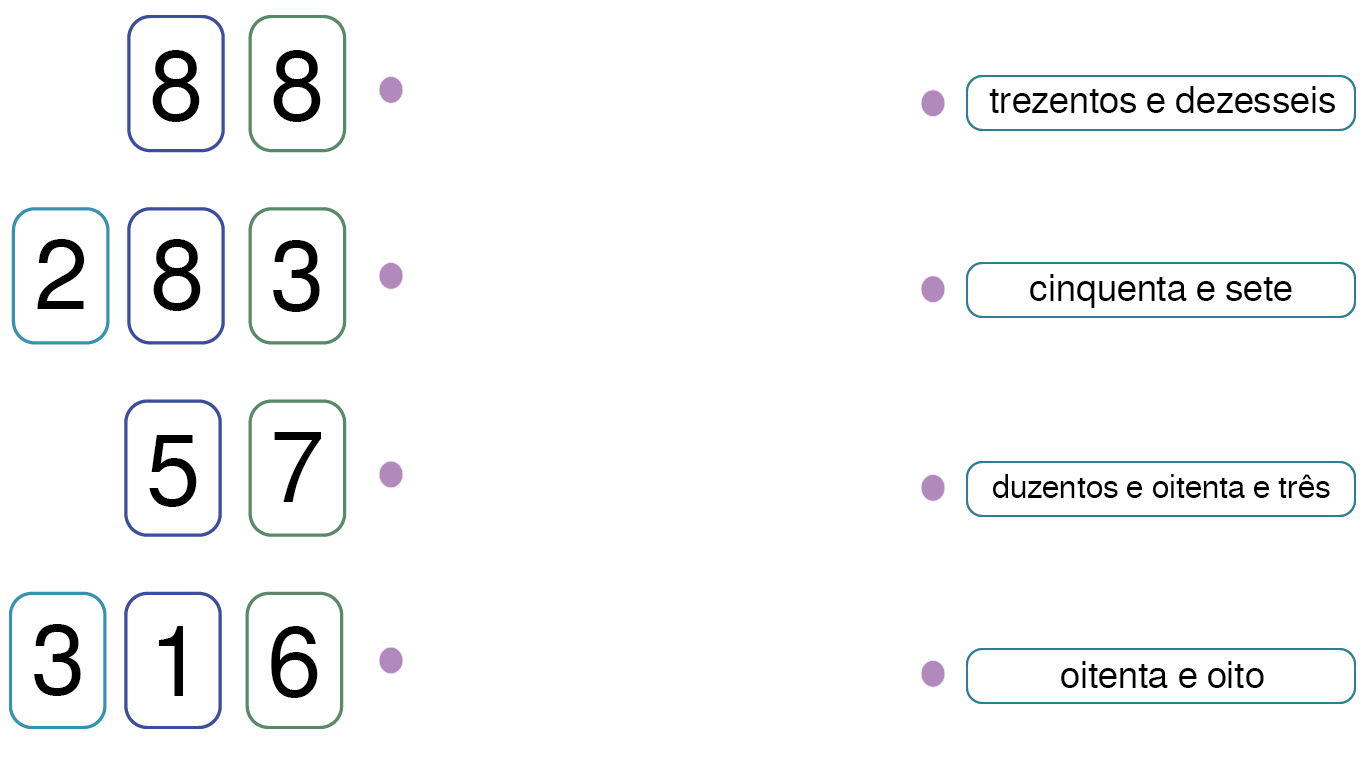
\includegraphics[width=4.89702in,height=6.12128in]{media/image5.png}

Disponível
em:\textless https://www.eunapolis.ba.gov.br/site/Noticias/noticia-060220221925071633-Vacina-o-Covid-19-para-crian-as-de-5-a-11-anos
Acesso em: 05 abr 2023

Nesta campanha, pode-se notar que o discurso persuasivo pretende
informar sobre a importância das vacinas em crianças afirmando que todo
argumento contrário à vacinação é irresponsabilidade. Neste caso, a
campanha faz uso de um jogo de palavras que rimam e fazem parte do
discurso informal, trazendo ideia de proximidade com o público alvo. As
palavras usadas para chamar a atenção para o assunto são:

\begin{enumerate}
\def\labelenumi{\alph{enumi})}
\item
  Filhos e família
\item
  Menores e responsabilidade
\item
  Pai ou mãe
\item
  Vacine e Vacile
\end{enumerate}

Identificar o uso de recursos persuasivos em textos verbais e não
verbais

a) Incorreta. Embora as palavras apareçam e chamem a atenção não são os
principais recursos

b) Incorreta. Estas palavras aparecem mas têm importância secundária na
mensagem principal

c) Incorreta. Estas palavras aparecem mas têm importância secundária na
mensagem principal

d) Correta. O jogo com as palavras e o fato de estarem no imperativo são
responsáveis pela persuasão da peça

\textbf{Questão 3:}

CAPÍTULO I

DISPOSIÇÕES GERAIS

Art. 1º É instituída a Lei Brasileira de Inclusão da Pessoa com
Deficiência (Estatuto da Pessoa com Deficiência), destinada a assegurar
e a promover, em condições de igualdade, o exercício dos direitos e das
liberdades fundamentais por pessoa com deficiência, visando à sua
inclusão social e cidadania.

Parágrafo único. Esta Lei tem como base a Convenção sobre os Direitos
das Pessoas com Deficiência e seu Protocolo Facultativo, ratificados
pelo Congresso Nacional por meio do Decreto Legislativo nº 186, de 9 de
julho de 2008 , em conformidade com o procedimento previsto no § 3º do
art. 5º da Constituição da República Federativa do Brasil , em vigor
para o Brasil, no plano jurídico externo, desde 31 de agosto de 2008, e
promulgados pelo Decreto nº 6.949, de 25 de agosto de 2009 , data de
início de sua vigência no plano interno.

\href{https://www.planalto.gov.br/ccivil_03/_ato2015-2018/2015/lei/l13146.htm}{{https://www.planalto.gov.br/ccivil\_03/\_ato2015-2018/2015/lei/l13146.htm}}.
Acesso em 27 de Abr. de 2023

O texto acima pertence ao domínio dos textos normativos e tem como
objetivo assegurar os direitos das pessoas com deficiência. Esta
afirmação pode ser comprovada:

\begin{enumerate}
\def\labelenumi{\alph{enumi})}
\item
  Pelo artigo primeiro das disposições gerais
\item
  Pelo Artigo quinto da Constituição federal
\item
  Pelo capítulo I
\item
  Pelo parágrafo único
\end{enumerate}

Saeb:Identificar formas de organização de textos normativos, legais e/ou
reivindicatórios.

a) Correta. Logo no primeiro artigo aparecem as disposições gerais e os
temas a serem normalizados pela lei

b) Incorreta. O artigo quinto da Constituição aparece como refoço e
justificativa da importância da Lei

c) Incorreta. O capítulo primeiro compreende demais partes e
peculiaridades da Lei

d) Incorreta. O parágrafo único apresenta as justificativas sobre
pertinência da regulamentação do Estatuto da Pessoa com Deficiência

\textbf{Questão 4:}

Aqui em Manaus faço uma parte desse grande projeto que é desenvolvido
por diversas instituições japonesas e conta com financiamento da GHIT
Funding, tendo à frente o doutor Shigeto Yoshida, da Universidade de
Kanazawa {[}Japão{]}, que é o desenvolvedor dessa formulação vacinal.
Essa vacina atua contra o parasita no hospedeiro humano e, também,
tentando evitar a infecção do hospedeiro que é o vetor, que transmite a
doença de uma pessoa para outra. Ela tem na sua forma a proteína CSP,
presente na vacina que já está em uso em diversos países da África e na
vacina desenvolvida pela Universidade de Oxford {[}Reino Unido{]}. Então
ela tem esse pedaço do parasita, essa proteína, que é um alvo estudado
já há muitos anos e com poder de proteção para as infecções nos humanos.
Essa proteína tem um papel importante para impedir que o parasita chegue
ao fígado, que é o primeiro local em que ele se instala, e, por causa
disso, os anticorpos e a resposta celular produzidos por uma vacina
poderiam impedir a entrada do parasita e seu desenvolvimento nos
humanos.

\href{https://cienciahoje.org.br/artigo/malaria-uma-vacina-contra-um-desafio-amazonico/}{{https://cienciahoje.org.br/artigo/malaria-uma-vacina-contra-um-desafio-amazonico/}}.
Acesso em 27 de Abr de 2023

Neste texto, podemos ver a explicação de como devem funcionar as vacinas
contra a malária e como estão sendo desenvolvidas. São marcadores
discursivo de conclusão os seguintes termos:

\begin{enumerate}
\def\labelenumi{\alph{enumi})}
\item
  \ldots e, também,...
\item
  \ldots tendo à frente\ldots{}
\item
  Então\ldots{}
\item
  Por causa disso
\end{enumerate}

Identificar elementos constitutivos de gêneros de divulgação científica

a) Incorreta. O termo aparece na introdução do assunto

b) Incorreta. O termo não tem função de conclusão

c) Incorreta. Embora apareça na parte da conclusão e pudesse ser usado
com essa função, no caso o termo aparece como marca de oralidade

d) Correta. Correta. O termo pretende introduzir a conclusão a partir
das afirmações e esclarecimentos já expressos.

\textbf{Questão 5:}

\textbf{Exemplo 1:}

A relação do ser humano com os animais de estimação existe há mais de 10
mil anos. Os animais domésticos preenchem várias necessidades emocionais
dos homens e dessa forma esses bichinhos, principalmente cães e gatos,
se tornam cada vez mais parte da nossa casa e de nossa família.

Mas infelizmente, muita gente ainda possui animais de estimação, mas não
possui a menor condição de cria-los. E quando falamos em condição de
criar, refiro-me principalmente a condições psicológicas.

Tanto é verdade que os maus-tratos aos `pets' são evidentes em todas as
cidades do país: animais famintos, torturados, feridos covardemente,
confinados em espaços minúsculos ou abandonados nas ruas ou estradas
Brasil afora.

E se quisermos mudar essa situação, precisamos perder o medo e o receio
de nos envolver e denunciar os maus-tratos, pois os mesmos só cessarão
quando aqueles que cometem esses crimes começarem a ser exemplarmente
punidos.

\href{https://www.jornalcidademg.com.br/artigo-os-maus-tratos-e-o-abandono-de-animais/}{\textbf{{https://www.jornalcidademg.com.br/artigo-os-maus-tratos-e-o-abandono-de-animais/}}}

\textbf{Exemplo 2:}

\textbf{Polícia resgata 10 cachorros em situação de maus-tratos em dois
imóveis de Curitiba}

Resgate aconteceu no bairro Abranches e no Barreirinha. Polícia chegou
aos casos após denúncias de vizinhos.

A Polícia Civil e a Rede de Proteção Animal de Curitiba resgataram 10
cachorros que estavam em situação de maus-tratos na capital paranaense,
na quinta-feira (23).

O resgate aconteceu em dois imóveis, um no bairro Abranches e outro no
Barreirinha.

O proprietário do imóvel do Abranches foi multado em R\$ 12 mil, por
criação e venda irregulares e maus-tratos aos animais. A suspeita é que
no local existia um criadouro ilegal.

https://g1.globo.com/pr/parana/noticia/2023/02/24/policia-resgata-10-cachorros-em-situacao-de-maus-tratos-em-dois-imoveis-de-curitiba.ghtml

Os dois exemplos foram extraídos de meios de comunicação e representam
diferentes gêneros do campo jornalístico. Com base nas diferenças entre
os dois textos é correto afirmar que:

\begin{enumerate}
\def\labelenumi{\alph{enumi})}
\item
  O exemplo 1 é uma entrevista e o exemplo dois é uma notícia
\item
  O exemplo 1 é um artigo de opinião e o exemplo 2 uma notícia
\item
  O exemplo 1 é uma reportagem e o exemplo 2 um artigo de opinião
\item
  O exemplo 1 é uma carta de leitor e o exemplo 2 é um artigo de opinião
\end{enumerate}

Analisar a relação temática entre diferentes gêneros jornalísticos.

a) Incorreta. O exemplo 1 não apresenta traços de entrevista

b) Correta. O exemplo 1 representa um artigo de opinião pois apresenta
argumentação acerca do tema e o exemplo 2 é uma notícia pois está
dividido em título, linha fina, lide e corpo

c) Incorreta. O exemplo 1 não é uma reportagem pois apresenta
argumentação e expõe opiniões do autor e o exemplo 2 não é um artigo de
opinião pois apresenta um fato com alto grau de imparcialidade e
objetividade

d) Incorreta. O exemplo 1 não apresenta formas de composições próprias
do gênero de carta do leitor e o exemplo 2 não emite opinião

\textbf{Questão 6:}

Apartava se Nise de Montano,

em cuja alma partindo se ficava;

que o pastor na memória a debuxava,

por poder sustentar-se deste engano.

Pelas praias do Índico Oceano

sobre o curvo cajado se encostava,

e os olhos pelas águas alongava,

que pouco se doíam de seu dano.

Pois com tamanha mágoa e saudade

(dizia) quis deixar me a que eu adoro,

por testemunhas tomo Céu e estrelas.

Mas se em vós, ondas, mora piedade,

levai também as lágrimas que choro,

pois assim me levais a causa delas!

CAMÕES, Luís Vaz de. Os Lusíadas de Luís Camões. Direção Literária Dr.
Álvaro Júlio da Costa Pimpão.

\href{http://www.dominiopublico.gov.br/download/texto/bv000164.pdf}{{http://www.dominiopublico.gov.br/download/texto/bv000164.pdf}}.
Acesso em 27de Abr. de 2023

Considerando os elementos que caracterizam os textos literários, o texto
acima pode ser considerado:

\begin{enumerate}
\def\labelenumi{\alph{enumi})}
\item
  Conto, pois apresenta poucos personagens e se desenvolve em espaço
  limitado
\item
  Texto dramático, pois faz referência aos sentimentos dos personagens e
  suas ações
\item
  Poema, pois está dividido em versos e estrofes e a métrica apresentada
  o caracteriza como um soneto
\item
  Romance, pois narra a relação de saudade e mágoa dos personagens e
  narra uma história longa
\end{enumerate}

Analisar elementos constitutivos de textos pertencentes ao domínio
literário.

a) Incorreta. O texto não apresenta características de conto

b) Incorreta. O texto não apresenta os personagens, suas falas e
tampouco rubrica

c) Correta. O texto é um poema a forma de composição em quatro estrofes,
sendo as duas primeiras contendo 4 versos e as duas últimas 3 versos o
caracterizam como um soneto

d) Incorreta. O texto não é um romance, não apresenta narrador nem
enredo longo

\textbf{Questão 7:}

\textbf{Falta de iluminação em rua completa 1 ano e tem 'festa de
aniversário' como protesto em Ourinhos}

Manifestação foi na Rua Narciso Nicolosi no Jardim Paulista. Prefeitura
informou na manhã seguinte ao ato que fez a troca de lâmpada queimada.

Moradores de Ourinhos (SP) protestaram contra a falta de iluminação
pública na Rua Narciso Nicolosi, no Jardim Paulista, na noite desta
quarta-feira (26) com uma "festa de aniversário" para marcar um ano de
espera pela troca de lâmpadas em um poste.

A ``comemoração'' teve bolo com vela, refrigerante, bexigas, cartazes e
parabéns para você em coro e palmas em meio a críticas pela escuridão.

Os termos entre aspas na notícia indicam:

\begin{enumerate}
\def\labelenumi{\alph{enumi})}
\item
  Ironia, pois os termos estão sendo utilizados de forma provocativa
\item
  Citação de falas de autoridades da cidade
\item
  Citação de argumentos de especialistas
\item
  Ênfase nas palavras e termos destacados
\end{enumerate}

Analisar efeitos de sentido produzido pelo uso de formas de apropriação
textual (paráfrase, citação etc.).

a) Correta. Os termos estão sendo usados de forma irônica para protestar
contra a falta de energia

b) Incorreta. O uso de aspas neste caso não pretende indicar a fala de
autoridades

c) Incorreta. O uso das aspas neste caso não pretende introduzir falas
de especialistas

d) Incorreta. Os termos não estão sendo puramente enfatizados, o uso de
aspas se dá principalmente pelo contexto irônico da notícia

\textbf{Questão 8:}

\textbf{Telegram diz que Justiça ordenou entrega de dados `impossíveis'
de serem obtidos; PF afirma que lentidão permitiu exclusão de
informações}

Cofundador do aplicativo afirmou que empresa está recorrendo da
suspensão do serviço, que começou a valer na noite da última quarta
(26).

O cofundador do Telegram Pavel Durov afirmou nesta quinta-feira (27) que
a Justiça brasileira ordenou a entrega de dados "impossíveis" de serem
coletados. Em seu canal no aplicativo, ele afirmou que a empresa vai
recorrer da decisão.

\href{https://g1.globo.com/tecnologia/noticia/2023/04/27/telegram-diz-que-justica-ordenou-coleta-de-dados-impossiveis-de-serem-obtidos-pf-afirma-que-lentidao-permitiu-exclusao-de-informacoes.ghtml}{{https://g1.globo.com/tecnologia/noticia/2023/04/27/telegram-diz-que-justica-ordenou-coleta-de-dados-impossiveis-de-serem-obtidos-pf-afirma-que-lentidao-permitiu-exclusao-de-informacoes.ghtml}}.
Acesso em 27 de Abr. de 2023.

Analise o título da notícia e assinale a alternativa correta:

\begin{enumerate}
\def\labelenumi{\alph{enumi})}
\item
  O título da notícia expressa concordância do veículo de comunicação
  com a justificativa apresentada pela empresa
\item
  O título da notícia expressa discordância em relação ao argumento
  apresentado pela empresa
\item
  O título da notícia enfatiza a fala da defesa apresentada pela empresa
\item
  O título coloca o argumento em suspeita a validade do argumento
  apresentado pela empresa
\end{enumerate}

Analisar os efeitos de sentido decorrentes dos mecanismos de construção
de textos jornalísticos/midiáticos.

a) Incorreta. O título não expressa concordância nem discordância quanto
ao argumento da empresa

b) Incorreta. O título não expressa concordância nem discordância quanto
ao argumento da empresa

c) Incorreta. O título não pretende enfatizar a fala da empresa em sua
defesa

d) Correta. O título apresenta ironia ao colocar em suspeição a validade
do argumento da empresa

\textbf{Questão 9:}

O RATO DO MATO E O RATO DA CIDADE

Um ratinho da cidade foi uma vez convidado para ir à casa

de um rato do campo. Vendo que seu companheiro vivia pobremente de
raízes e ervas, o rato da cidade convidou-o a ir morar com ele:

--- Tenho muita pena da pobreza em que você vive --- disse.

ABREU, Ana Rosa{[}et al.{]}Alfabetização: livro do aluno Brasília :
FUNDESCOLA/SEFMEC, 2000. p. 102.

\href{http://www.dominiopublico.gov.br/download/texto/me001614.pdf}{{http://www.dominiopublico.gov.br/download/texto/me001614.pdf}}
Acesso em 27 de Abr de 2023.

A partir do trecho acima é possível afirmar que:

\begin{enumerate}
\def\labelenumi{\alph{enumi})}
\item
  O rato do campo vivia confortável e muita comida disponível
\item
  O rato da cidade era muito pobre e não tinha o que comer
\item
  Os dois ratinhos possuíam os mesmos confortos e acesso a alimentação
\item
  O rato da cidade tinha mais conforto e acesso a comida que o rato do
  campo
\end{enumerate}

Inferir informações implícitas em distintos textos

\begin{enumerate}
\def\labelenumi{\alph{enumi})}
\item
  Incorreta. O trecho destaca a escassez na qual vivia o rato do campo
\item
  Incorreta. O rato pobre era o rato do campo
\item
  Incorreta. O trecho destaca a escassez na qual vivia o rato do campo
\item
  Correta. O trecho traz a informação de que o rato do campo vivia com
  grandes dificuldades. Com pena, o rato da cidade convidou-o para morar
  com ele, deixando implícito que na cidade teriam mais conforto e
  acesso a comida
\end{enumerate}

\textbf{Questão 10:}

Os recifes de coral são ambientes extremamente diversos, abrigando cerca
de 25\% de toda a biodiversidade marinha. Suas estruturas rígidas são
constituídas por organismos marinhos de esqueleto calcário, os corais.
Mas há outros tipos de organismos que vivem nos recifes, como algas,
moluscos e peixes.

Além de sua importância biológica, recifes também são valiosos do ponto
de vista socioeconômico. A elevada biodiversidade produz bastante
pescado, de modo que, hoje, cerca de 10\% da proteína animal consumida
no planeta provêm de recifes de coral. Outro fator a considerar é que a
beleza natural estimula o turismo, e, consequentemente, o
estabelecimento de operadoras de mergulho, pousadas,
restaurantes\ldots{}
https://cienciahoje.org.br/artigo/recifes-sob-estresse/ Acesso em 27 de
Abr de 2023.

A importância biológica dos recifes de coral pode ser comprovada por:

\begin{enumerate}
\def\labelenumi{\alph{enumi})}
\item
  Por conterem beleza natural que estimula o turismo e o comércio de
  pousadas e restaurantes
\item
  Por serem estruturas rígidas constituídas por organismos marinhos de
  esqueleto calcário, chamadas de corais.
\item
  Por serem ambientes extremamente diversos, abrigando cerca de 25\% de
  toda a biodiversidade marinha.
\item
  Por contribuírem com a presença de peixes favorecendo a produção de
  pescado
\end{enumerate}

Distinguir fatos de opiniões em textos.

a) Incorreta. Este não é argumento que apoia a factualidade da afirmação

b) Incorreta. Esta não é a característica que comprova a afirmação

c) Correta. Segundo o texto, os recifes de corais são importantes
biologicamente por abrigarem grande biodiversidade

d) Incorreta. Esta característica sustenta seu valor socioeconômico

\textbf{Questão 11:}

Algumas atitudes da sociedade têm colaborado para que as crianças
desenvolvam hábitos alimentares saudáveis. É o caso de escolas que
procuram controlar o tipo de comida consumida pelos seus alunos. Na
cantina ou lancheira são proibidos doces e frituras. Caso a criança os
traga de casa, ele é mandado de volta e uma outra solução é dada para a
refeição daquele dia.

Mesmo assim, alguns pais acabam infringindo as regras e mandando como
lanche para seus filhos alguns alimentos proibidos. Muitos justificam
que se não for aquilo, a criança não come, sendo melhor que coma algo
sem qualidade que ficar de estômago vazio.

\href{https://g1.globo.com/educacao/noticia/2010/04/opiniao-alimentacao-saudavel-na-mira-das-escolas-e-dos-pais.html}{{https://g1.globo.com/educacao/noticia/2010/04/opiniao-alimentacao-saudavel-na-mira-das-escolas-e-dos-pais.html}}.
Acesso em 27 de Abr de 2023

No último parágrafo do texto o autor deixa claro que:

\begin{enumerate}
\def\labelenumi{\alph{enumi})}
\item
  A escola não se empenha em promover uma alimentação saudável para os
  estudantes
\item
  Os pais se empenham em promover uma alimentação saudável para os
  filhos
\item
  Tanto os pais quanto as escolas estão empenhados em oferecer uma
  alimentação saudável para os filhos e estudantes
\item
  Apesar das restrições e atitudes da escola, alguns pais não se
  empenham em oferecer uma alimentação saudável para os filhos
\end{enumerate}

Analisar os processos de referenciação lexical e pronominal.

a) Incorreta. O texto afirma a atitude da escola em relação à promoção
de uma alimentação saudável para os estudantes

b) Incorreta. O texto não afirma que exista uma atitude positiva dos
pais em relação `alimentação dos filhos

c) Incorreta. O texto afirma a atitude positiva da escola e questiona a
atitude dos pais com relação à alimentação dos estudantes

d) Correta. O uso da expressão `mesmo assim' deixa claro que apesar dos
esforços da escola alguns pais não ajudam a promover uma alimentação
mais saudável para os filhos

\textbf{Questão 12:}

\textbf{Direito da criança de brincar na rua é negligenciado}

\emph{Carimba, cabra-cega, passa anel, boca-de forno, batata-quente.
Crianças desconhecem muitas brincadeiras}

Simplesmente brincar. Na rua, nas praças, quadras, parquinho, com
amigos, com vizinhos. É direito constitucional, está nos estatutos,
declarações e lei. Mas, efetivamente, a brincadeira está bem longe de
ser uma prioridade, tanto para muitas crianças, quanto para os pais.

\href{https://diariodonordeste.verdesmares.com.br/metro/direito-da-crianca-de-brincar-na-rua-e-negligenciado-1.621061}{{https://diariodonordeste.verdesmares.com.br/metro/direito-da-crianca-de-brincar-na-rua-e-negligenciado-1.621061}}.
Acesso em 27 de Abr de 2023

Ao analisar a reportagem pode- se afirmar que há marca de parcialidade
no trecho:

\begin{enumerate}
\def\labelenumi{\alph{enumi})}
\item
  Simplesmente brincar.
\item ~
  \hypertarget{direito-da-crianuxe7a-de-brincar-na-rua-uxe9-negligenciado}{%
  \section{Direito da criança de brincar na rua é
  negligenciado}\label{direito-da-crianuxe7a-de-brincar-na-rua-uxe9-negligenciado}}
\item
  Na rua, nas praças, quadras, parquinho, com amigos, com vizinhos.
\item
  É direito constitucional, está nos estatutos, declarações e lei
\end{enumerate}

Avaliar diferentes graus de parcialidade em textos jornalísticos

a) Incorreta. O trecho não apresenta parcialidade

b) Correta. O título da notícia expressa a opinião de que o direito de
brincar é negligenciado

c)Incorreta. O trecho não apresenta parcialidade

d) Incorreta. O trecho não apresenta parcialidade pois se apoia em fatos

\textbf{Questão 13:}

\textbf{Strava mostra aumento do número de ciclistas, pós pandemia, em
seis capitais}

A pandemia trouxe algumas mudanças positivas que têm tudo para se tornar
permanentes para muitas pessoas. Uma delas foi o maior número de
ciclistas pelas cidades, que começaram a utilizar o meio de locomoção
com o receio de compartilhar viagens em carros e transportes urbanos.

\href{https://www.otempo.com.br/opiniao/esportivamente/strava-mostra-aumento-do-numero-de-ciclistas-pos-pandemia-em-seis-capitais-1.2571161.Acesso}{{https://www.otempo.com.br/opiniao/esportivamente/strava-mostra-aumento-do-numero-de-ciclistas-pos-pandemia-em-seis-capitais-1.2571161}}.
Acesso em 27 de Abr de 2023

Na primeira parte do texto o uso da expressão ``têm tudo para se
tornar\ldots'' representa:

\begin{enumerate}
\def\labelenumi{\alph{enumi})}
\item
  Um otimismo do autor em relação manuntenção das mudanças positivas
  impostas pela pandemia
\item
  Um pessimismo do autor em relação a continuidade das atitudes
  positivas impulsionadas pela pandemia
\item
  Uma posição neutra em relação às mudanças positivas que chegaram com a
  pandemia
\item
  Uma condição para que as mudanças positivas impostas pela pandemia se
  perpetuem
\end{enumerate}

Identificar os recursos de modalização em textos diversos.

a) Correta. O autor expressa por meio deste recurso de modalização que a
adoção de certas atitudes têm grandes chances permanecem

b) Incorreta. A expressão indica otimismo

c) Incorreta. A expressão sugere o posicionamento do autor

d) Incorreta. O termo não sugere condição, apenas aponta alguns fatores
favoráveis

\textbf{Questão 14:}

A Academia Americana de Medicina do Sono recomenda que crianças e
adolescentes entre 6 e 12 anos durmam ao menos nove horas por dia, mas
muitos não seguem a recomendação e os pesquisadores queriam entender
melhor o impacto de menos horas de descanso no desenvolvimento desses
jovens.

Os cientistas analisaram os dados de 8.323 crianças de 9 e 10 anos. Eles
dividiram esse conjunto em dois grupos das crianças que dormiam menos de
nove horas (4.181 participantes) e daquelas que dormiam pelo menos nove
horas (4.142 participantes)- e avaliaram seus dados neurais e
comportamentais no início da pesquisa e após dois anos.

Os cientistas notaram também uma diferença significativa no volume de
massa cinzenta em 12 das 184 regiões avaliadas, padrão que se repetiu
depois de dois anos, sugerindo que algumas medidas estruturais são
suscetíveis a períodos insuficientes de sono.

\href{https://www.otempo.com.br/mundo/dormir-menos-de-nove-horas-afeta-cerebro-e-comportamento-das-criancas-1.2707918}{{https://www.otempo.com.br/mundo/dormir-menos-de-nove-horas-afeta-cerebro-e-comportamento-das-criancas-1.2707918}}.
Acesso em 27 de Abr de 2023

No texto acima a principal estratégia de argumentação se dá por meio de:

\begin{enumerate}
\def\labelenumi{\alph{enumi})}
\item
  falas de especialistas e opiniões de pais
\item
  discurso de autoridade e citação de fontes confiáveis
\item
  contraste e exemplos históricos
\item
  exemplos e dados de pesquisas
\end{enumerate}

Avaliar a eficácia das estratégias argumentativas em textos de
diferentes gêneros.

\begin{enumerate}
\def\labelenumi{\alph{enumi})}
\item
  Incorreta. O texto não apresenta falas de especialistas
\item
  Incorreta. Não há citação de fontes e discursos de autoridade no
  trecho
\item
  Incorreta. Não há argumentos por contraste e tampouco exemplos
  históricos
\item
  Correta. O texto se apoia em dados de pesquisas e exemplos reais de
  casos estudados
\end{enumerate}

\textbf{Questão 15:}

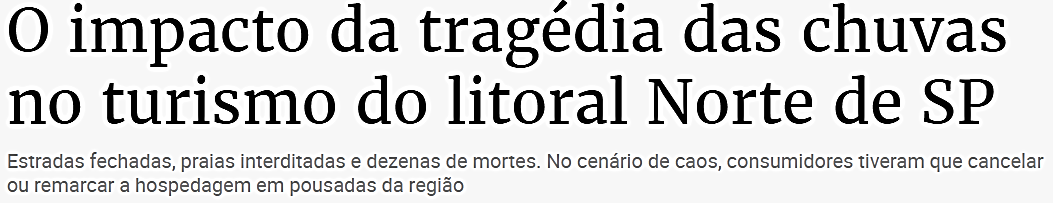
\includegraphics[width=2.84494in,height=2.84494in]{media/image6.png}

\href{https://www.justicaeleitoral.jus.br/jovem-eleitor/?fbclid=IwAR2KcQkYHtNdGnJHOLBrdsiujGlgHJ2bl39bYsMkNucRC48e5zyZwrpXbTo}{{https://www.justicaeleitoral.jus.br/jovem-eleitor/?fbclid=IwAR2KcQkYHtNdGnJHOLBrdsiujGlgHJ2bl39bYsMkNucRC48e5zyZwrpXbTo}}.
Acesso em 20 de Abr de 2023

A campanha acima é destinada ao público jovem e utiliza de recursos
verbais e não verbais para atingir este público alvo. Um recurso de
persuasão destinado a esse público pode ser lido em:

\begin{enumerate}
\def\labelenumi{\alph{enumi})}
\item
  Faltam 5 dias para a semana do Jovem Eleitor
\item
  Se você tem 15 anos completos ou 17
\item
  Tá por dentro?
\item
  A justiça eleitoral te dá uma forcinha para fazer seu 1º título
\end{enumerate}

Avaliar a adequação das variedades linguísticas em contextos de uso.

a) Incorreta. Este trecho não apresenta marca de variedade linguística

b) Incorreta. Este trecho não apresenta marca de variedade linguística

c) Correta. O uso de linguagem coloquial indica traço de variedade
linguística que funciona como recurso de persuasão destinado ao público
jovem

d) Incorreta. Este trecho não apresenta marca de variedade linguística
